% No compression; prevents errors when viewing PDF on Windows
\pdfobjcompresslevel=0

\documentclass[12pt]{article}

\usepackage{mathptmx,times}
\usepackage{amsmath}
\usepackage{tabularx}
\usepackage{booktabs, ragged2e, array, dcolumn}
\usepackage[font=small,format=plain,labelfont=bf,up]{caption}
\usepackage{enumitem}

\setlength{\textwidth}{6.5in}
\setlength{\textheight}{8.5in}
\setlength{\topmargin}{0in}
\setlength{\headheight}{0.25in}
\setlength{\headsep}{0.5in}
\setlength{\parindent}{0.25in}
\setlength{\oddsidemargin}{0in}
\setlength{\evensidemargin}{0.0in}
\setlength{\voffset}{-0.4in}
\setlength{\footskip}{0.5in}
\setlength{\marginparpush}{7pt}

\usepackage{titlesec}
\usepackage{graphicx}
\usepackage{floatrow}

\titlelabel{\thetitle.\quad}
\titleformat*{\section}{\bf\normalsize}
\titleformat*{\subsection}{\bf\normalsize}

\begin{document}

\begin{flushright}
\textbf{PBNC2014-218}
\end{flushright}

\begin{center}
\textbf{COMBINED FIRE MODEL UNCERTAINTY AND INPUT PARAMETER UNCERTAINTY ANALYSIS FOR NUCLEAR POWER PLANT SCENARIOS}
% \textbf{A MONTE CARLO ANALYSIS OF THE EFFECT OF FIRE SEVERITY ON NUCLEAR SAFETY STRUCTURES, SYSTEMS, AND COMPONENTS}
\end{center}

\begin{center}
\textbf{M. Clouthier\textsuperscript{1}, K. Overholt\textsuperscript{2}}\\

\textsuperscript{1}Clouthier Risk Engineering, Nova Scotia, Canada\\
\textsuperscript{2}National Institute of Standards and Technology, Gaithersburg, MD, USA
\end{center}

\begin{center}
\textbf{Abstract}
\end{center}

Quantitative fire risk analysis is used in conducting safety assessments at nuclear facilities to evaluate the potential consequences of postulated fire scenarios.

In fire modelling applications, the key phenomena that influence the predicted figure of merit (i.e., the specific objective of the analysis) are known; however, in some cases the existing state of knowledge and the adequacy of existing modelling tools to predict a given phenomenon is in need of improvement. It is therefore necessary to consider relevant uncertainties in a rational quantitative manner.

In this paper, a Monte Carlo analysis is applied to a fire scenario involving potential damage to nuclear safety structures, systems, and components. The effect of deterministic peak heat release rate and fire growth on the predicted hot gas layer is studied. The results of the case study are presented to demonstrate an improved method to develop a design basis fire.

\section{Introduction}
\label{sec:introduction}

% !TEX root = PBNC_Paper.tex

The area of uncertainty analysis is well established in science and engineering \cite{Morgan}.  Its role is to provide insight on the impact of uncertainties associated with engineering evaluations, which allows for meaningful and defensible decision making in risk assessment.

The practice of uncertainty analysis in fire modelling is evolving and the methodology employed is currently left to the practitioners' discretion. Often, a bounding analysis approach is taken, based on the assumption that uncertainty is addressed by specifying conservative values for input parameters. In some cases, bounding analysis by adopting a series of conservative assumptions as a substitute for uncertainty analysis could result in overly conservative decisions or provide a false understanding of the actual margin of safety. 

Uncertainty is addressed in fire protection engineering literature \cite{Notarianni:SFPE}.  And treatment of uncertainty analysis is explicitly required in most technical standards related to fire safety at nuclear power generating stations \cite{NFPA:805, NUREG:6850}.  Model bias and uncertainty has been quantified in Nuclear Regulatory Commission (NRC) NUREG-1824~\cite{NUREG_1824_Sup_1} for a number of fire models which are commonly used in nuclear power plant applications. This information can be used as part of a specific methodology to evaluate model uncertainty  that is presented in NRC NUREG-1934~\cite{NUREG_1934}. 

The treatment of  uncertainty and sensitivity in NUREG-1934 includes a summary of a derivation for quantifying model uncertainty \cite{McGrattan2011a}, as well as specific calculation examples in Section 4.3. Parameter uncertainty and methods to deal with this kind of uncertainty are discussed separately in Section 4.4; a simple brute force method is shown in  a worked example that propagates a HRR distribution through an algebraic model for predicted flame height, and determines the probability of flames reaching a certain height.

Given that input parameter uncertainty and model uncertainty are a both addressed separately in NUREG-1934; an apparent logical extension of the methodologies presented would be to treat both kinds of uncertainty in a manner that shows the combined effect of both kinds of uncertainty.  It is the aim of this paper to provide practitioners with a straight-forward and practical example of combined model and input uncertainty uncertainty analysis for a zone fire modelling application. 

In this paper, we demonstrate the calculation of three cases for one worked example for a fire scenario that is typical for a nuclear power generating station: 1) the effect of model bias and uncertainty, 2) the effect of input parameter uncertainty, and 3) the combined effect of model bias/uncertainty and input parameter uncertainty. 



\section{Previous work}
\label{sec:previous_work}

% !TEX root = PBNC_Paper.tex

The subject of model uncertainty and input parameter uncertainty and sensitivity has been covered extensively in the literature \cite{Spiegel, Vose, Kumamoto, Haimes}.  And there are numerous studies specific to fire modelling \cite{Notarianni:SFPE,  NUREG_1824, McGrattan2011a, Notarianni:1999, Lundin, Hostikka:2003a, Upadhyay2008, FDS_Validation_Guide}.  

Researchers have explored different methods for assessing uncertainty and sensitivity in complex models. In terms of sensitivity of output parameters to input values, Iman and Helton \cite{Iman:1988} concluded that Monte Carlo sampling offered the best overall performance compared to other methods such as differential analysis or response surface replacements.

Hostikka and Rahkonen \cite{Hostikka:2003a} used Monte Carlo simulation and CFAST to evaluate model sensitivity to numerous  input parameters such as fire power and growth rate, compartment geometry, and ventilation. This work estimated probabilities in terms of time to failure of electric cables in a tunnel fire, and hot gas layer development  in a compartment due to an electrical cabinet fire. 

A technique for calculating the sensitivity in model outputs resulting  from input parameter uncertainty is provided in Volume 2 of NUREG-1824. This method, which is also described in the Fire Dynamics Simulator (FDS) Technical Reference Guide \cite{FDS_Validation_Guide}, involves quantifying the functional dependence of the input parameters, based on the governing mathematical equations or simple algebraic correlations. 

A method for calculating model uncertainty is derived by McGrattan and Toman \cite{McGrattan2011a} and summarized in \cite{FDS_Validation_Guide}. This method involves comparisons of model predictions with experimental measurements. The work by McGrattan and Toman \cite{McGrattan2011a} presents a derivation of formulae to calculate  a bias factor and a relative standard deviation for a given model. Key assumptions are: (1) Experimental measurements are normally distributed about the ``true'' values, and there is no associated experimental systematic bias; and, (2)  model predictions are normally distributed about the true values multiplied by a bias factor. This methodology was applied for a number of fire models and the results of the study are presented in NUREG-1824.

In this work, the approach taken to evaluate the affect of model uncertainty follows the method developed by McGrattan and Toman and uses the results provided for CFAST in NUREG-1824 \cite{NUREG_1824_Sup_1}. The Monte Carlo method was used to evaluate model input parameter uncertainty for a single parameter. This paper presents a worked example of model and input parameter uncertainty analysis for a consistent fire scenario at a  nuclear power plant.  Initially, input parameter and model uncertainty are considered separately. Then, a combined approach is taken where both kinds of uncertainty are treated together.
 
 
 

 
 
 
 
 






\section{Fire model scenario setup}
\label{sec:fire_model_scenario_setup}

Appendix B from NRC NUREG-1934~\cite{NUREG_1934} was selected for this example analysis. The Consolidated Model of Fire Growth and Smoke Transport (CFAST)~\cite{CFAST_Users_Guide_6} zone model was used. The compartment has dimensions of 26.5~m by 18.5~m by 6.1~m. The ambient temperature was specified as 20~$^\circ$C. The simulation time is 1~h. The wall and ceiling materials were specified as concrete with a thermal conductivity of XX~W/m-K, density of XX~kg/m$^3$, and specific heat of XX~J/g-K.


\section{Uncertainty analysis}
\label{sec:uncertainty_analysis}

Input: Gamma distribution from NUREG 6850~\cite{NUREG_6850}, with a 75th percentile HRR of 232~kW and a 98th percentile HRR of 1002~kW. This corresponds to the case of vertical cabinets with unqualified cable, fire in more than one cable bundle open doors.
Output: Threshold HGL temperature of 100~$^\circ$C.


\clearpage


\subsection{Case 1: Model bias and uncertainty}

This case only accounts for model bias and uncertainty. A HRR of 1002~kW was selected as the input fire size, which represents the 98th percentile HRR. A PDF and CDF of the input HRR distribution is shown in Fig.~\ref{fig:case_1_input_distributions}. The model bias $\delta$ for forced ventilation for the CFAST zone model is 1.15, and the model relative standard deviation $\widetilde\sigma_M$ is 0.20.

\textbf{Step 1}: Specify the input HRR and run CFAST to calculate the resulting HGL temperature.

For an input HRR of 1002~kW, the CFAST model predicts an HGL temperature of 90.7~$^\circ$C. The probability of exceeding the threshold HGL temperature can be calculated following the procedure described in NUREG~1934~\cite{NUREG_1934}.

\textbf{Step 2}: Subtract the ambient value of the HGL temperature (20~$^\circ$C) to determine the predicted temperature rise.
\begin{equation}
M = 90.7~^\circ\textrm{C} - 20~^\circ\textrm{C} = 70.7~^\circ\textrm{C}
\end{equation}

\textbf{Step 3}: Refer to Table XX of NUREG 1824 Supplement 1~\cite{NUREG_1824_Sup_1}, which indicates that, on average, CFAST overpredicts HGL temperatures in forced ventilation scenarios with a bias factor $\delta$ of 1.15. The adjusted model prediction is calculated as
\begin{equation}
\mu = \frac{M}{\delta} = \frac{70.7~^\circ\textrm{C}}{1.15} \approx 81.5~^\circ\textrm{C}
\end{equation}
Referring again to Table XX of NUREG 1824 Supplement 1~\cite{NUREG_1824_Sup_1}, calculate the standard deviation of the distribution as
\begin{equation}
\sigma = \widetilde\sigma_M \left( \frac{M}{\delta} \right) = 0.20 \left( \frac{70.7}{1.15} \right) \approx 12.3~^\circ\textrm{C}
\end{equation}
Figure~\ref{fig:case_1_output_distributions} shows the resulting PDF and CDF of the adjusted HGL temperature distribution.

\textbf{Step 4}: Calculate the probability that the actual HGL temperature would exceed 100~$^\circ$C as
\begin{equation}
\textrm{P}(T > 100~^\circ\textrm{C}) = \frac{1}{2} \textrm{erfc} \left( \frac{T - \mu}{\sigma \sqrt{2}} \right) = \frac{1}{2} \textrm{erfc} \left( \frac{100~^\circ\textrm{C} - 81.5~^\circ\textrm{C}}{12.3~^\circ\textrm{C} \sqrt{2}} \right) \approx 0.07
\end{equation}
For Case 1, the probability of exceeding the critical HGL temperature of 100~$^\circ$C was calculated as 0.07.


\clearpage


\begin{figure}[!ht]
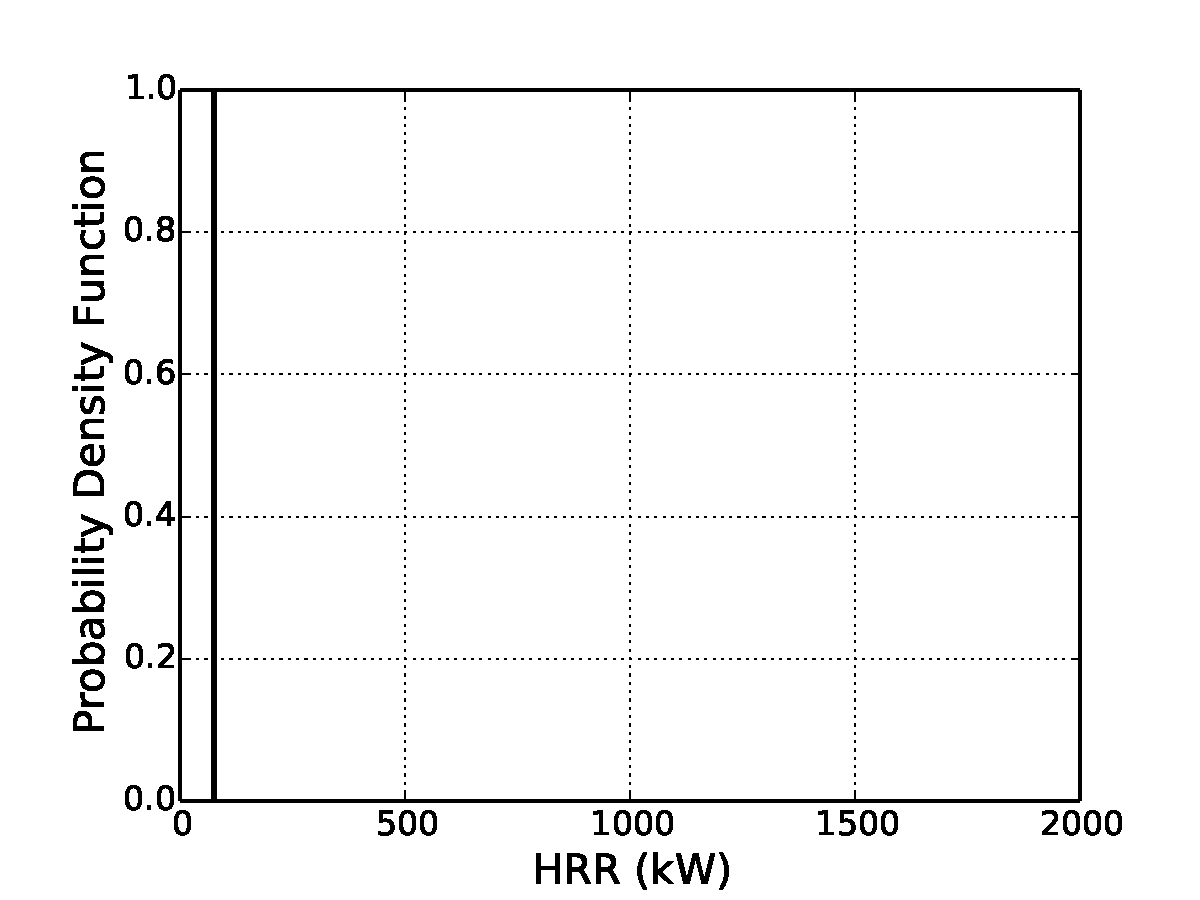
\includegraphics[width=2.6in]{Figures/input_PDF_point}
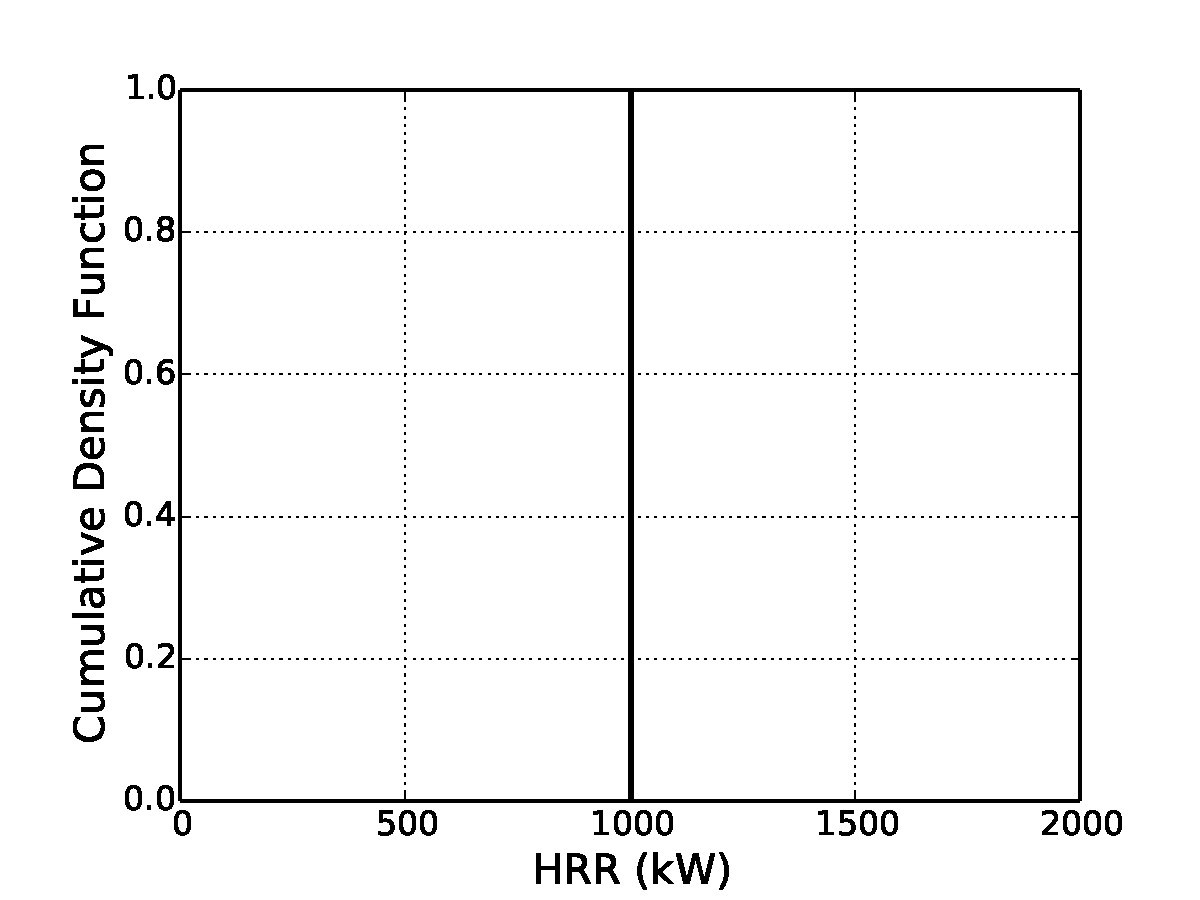
\includegraphics[width=2.6in]{Figures/input_CDF_point}
\caption{PDF and CDF of input HRR distribution}
\label{fig:case_1_input_distributions}
\end{figure}

\begin{figure}[!ht]
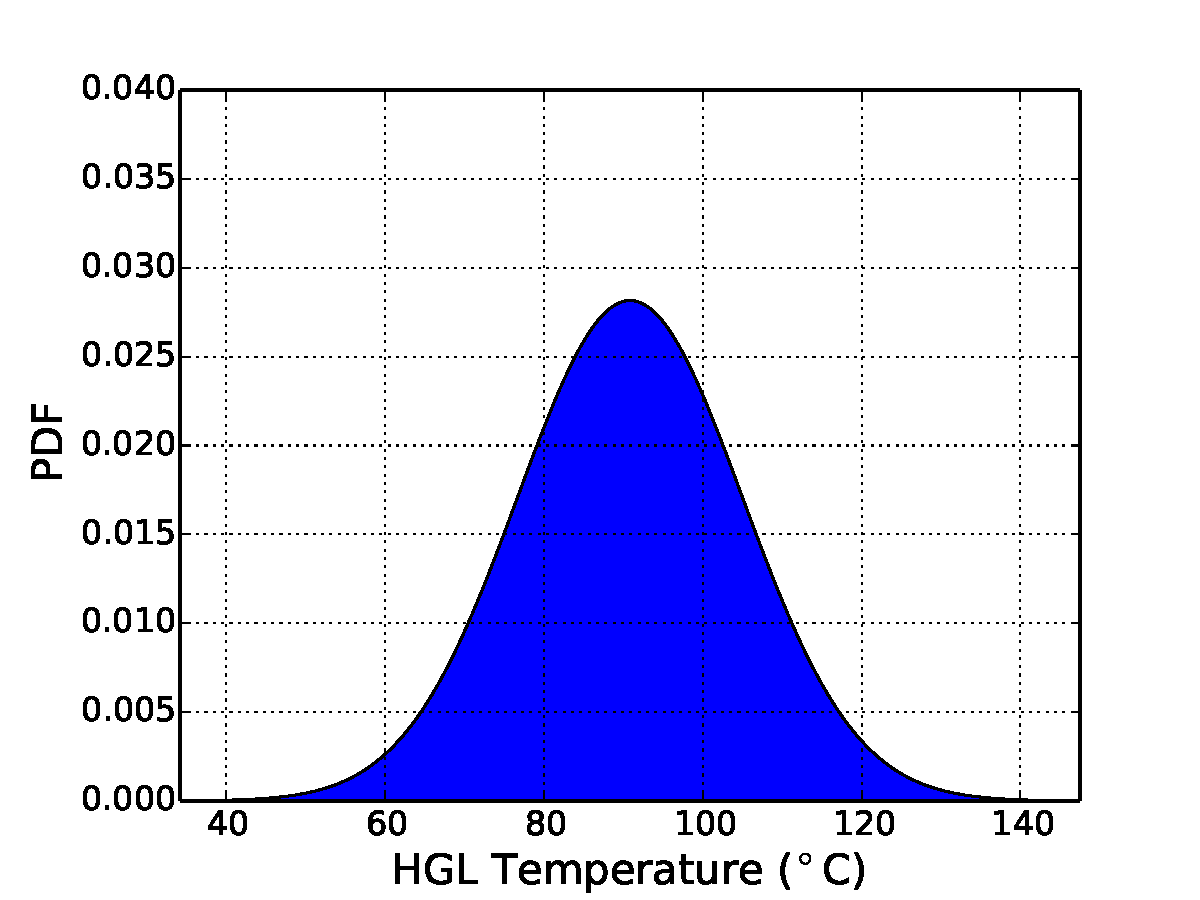
\includegraphics[width=2.6in]{Figures/output_PDF_1_model}
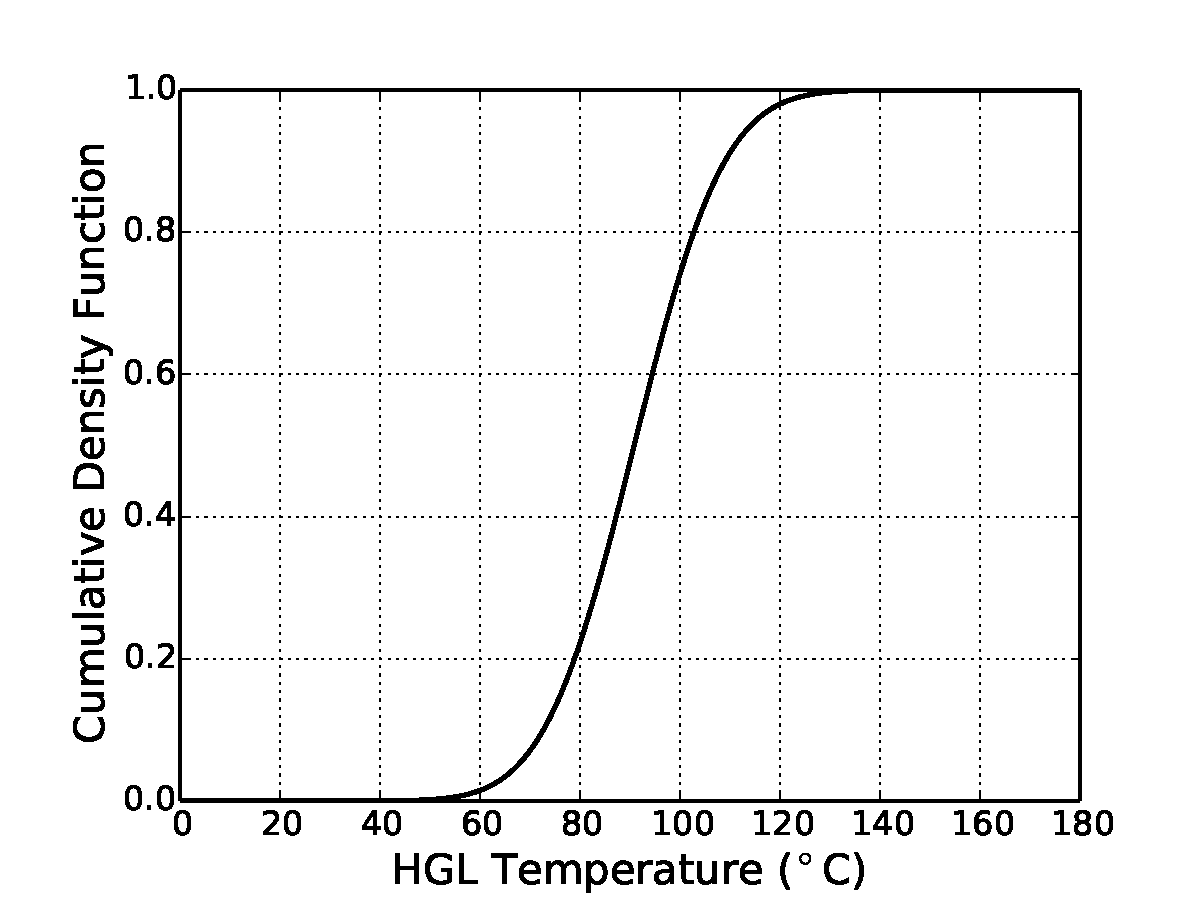
\includegraphics[width=2.6in]{Figures/output_CDF_1_model}
\caption{PDF and CDF of output HGL temperature distribution}
\label{fig:case_1_output_distributions}
\end{figure}


\clearpage


\subsection{Case 2: Input parameter uncertainty}

This case only accounts for input parameter uncertainty. Consider an gamma distribution for the HRR. Other distributions could be considered for the input parameter, such as a uniform or normal distribution.

\begin{enumerate}
\item Draw random sample from input distribution of HRRs.
\label{itm:case_2_step_1}
\item Run CFAST to calculate HGL temperature.
\item Store value and return to Step~\ref{itm:case_2_step_1}.
\item Calculate the probaility that the HGL temperature will exceed the threshold HGL temperature.
\end{enumerate}


\clearpage


A PDF and CDF of the input HRR distribution is shown in Fig.~\ref{fig:case_2_input_distributions}.

\begin{figure}[!ht]
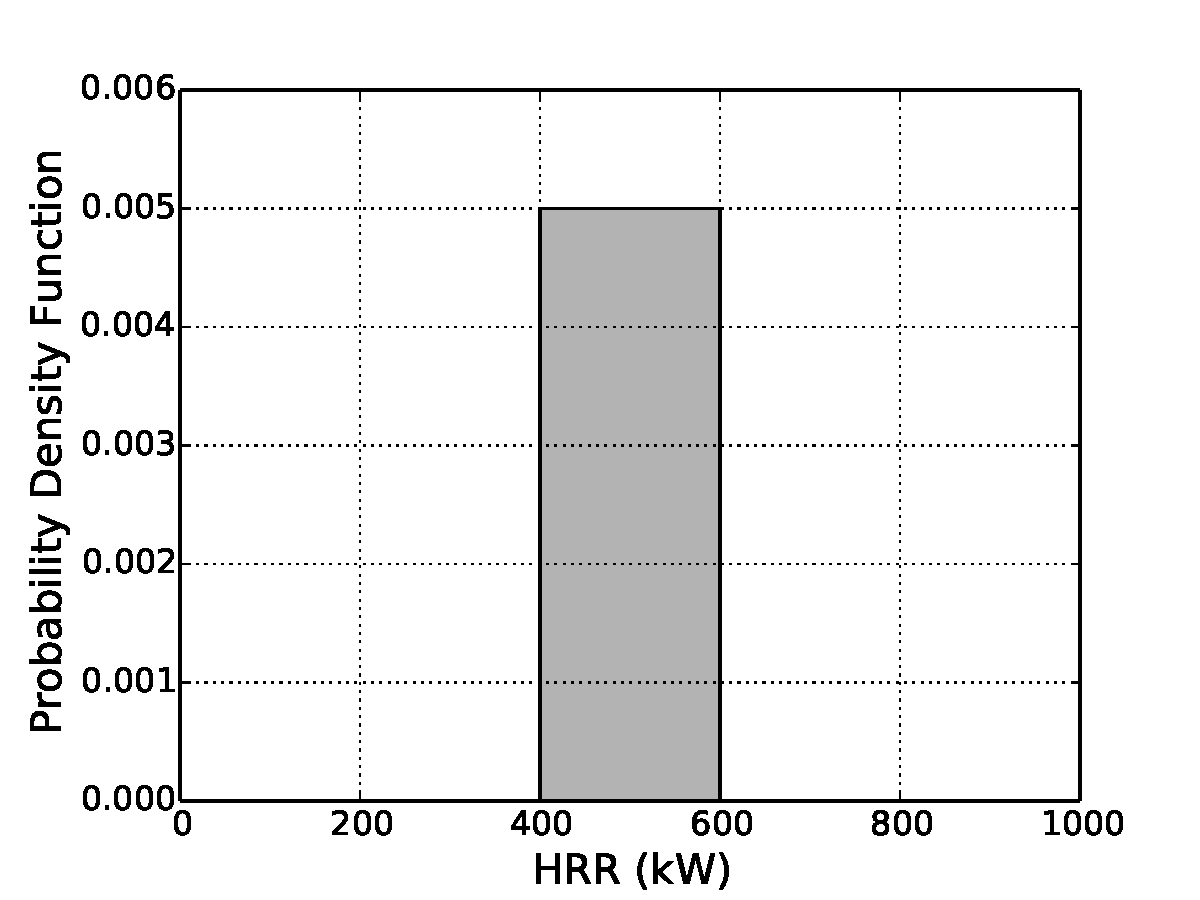
\includegraphics[width=2.6in]{Figures/input_PDF}
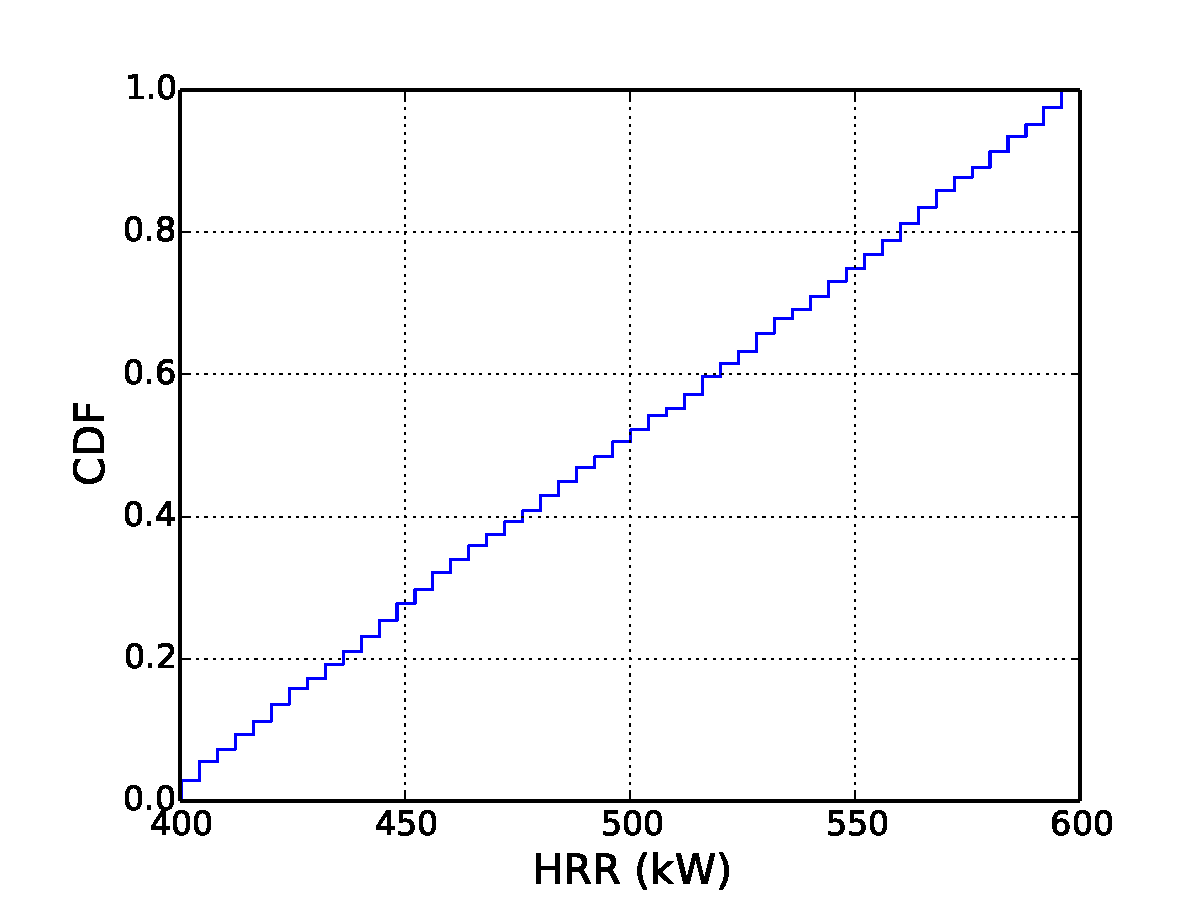
\includegraphics[width=2.6in]{Figures/input_CDF}
\caption{PDF and CDF of input HRR distribution}
\label{fig:case_2_input_distributions}
\end{figure}

The results of Case 2 are shown in Fig.~\ref{fig:case_2_output_distributions}.

\begin{figure}[!ht]
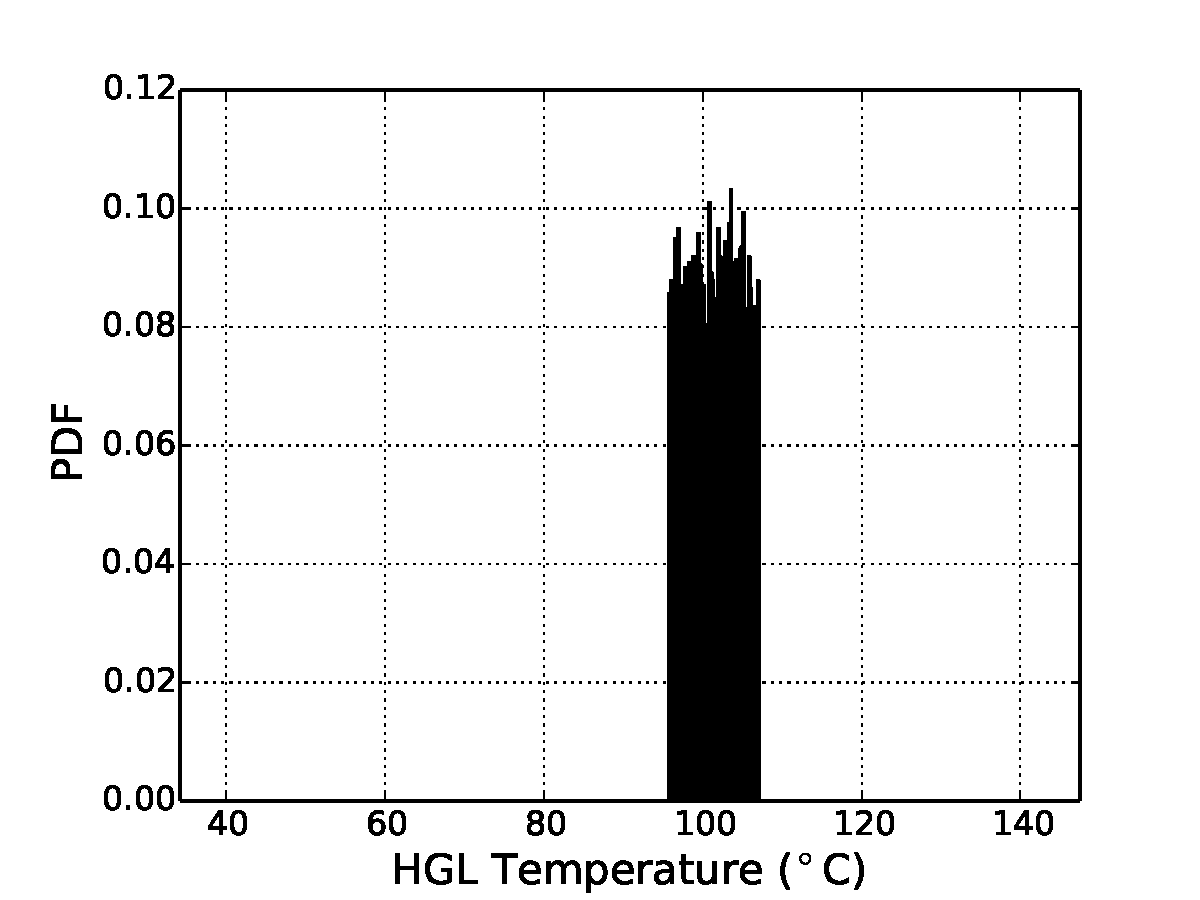
\includegraphics[width=2.6in]{Figures/output_PDF_2_input}
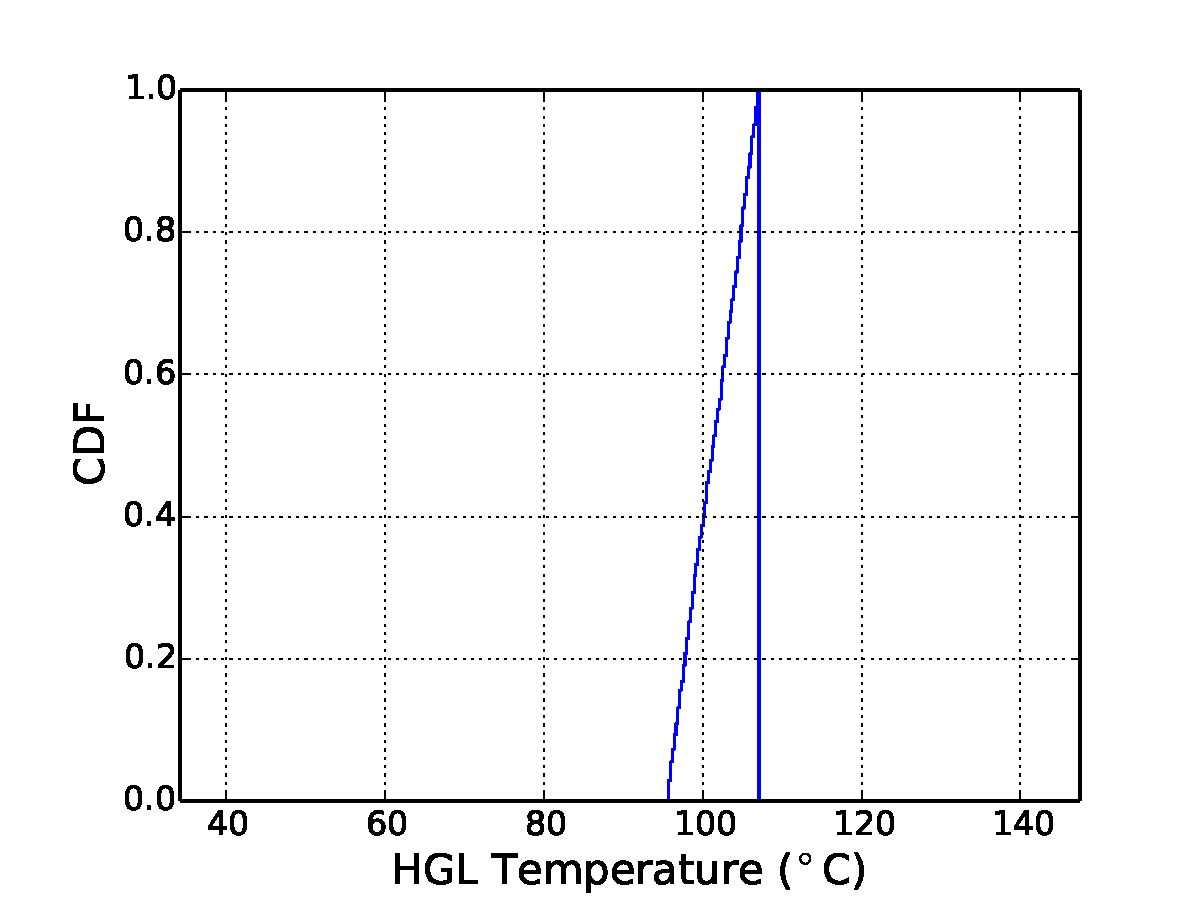
\includegraphics[width=2.6in]{Figures/output_CDF_2_input}
\caption{PDF and CDF of output HGL temperature distribution}
\label{fig:case_2_output_distributions}
\end{figure}

For Case 2, the probability of exceeding the critical HGL temperature of 100~$^\circ$C is calculated as XX.


\clearpage


\subsection{Case 3: Combined model and input parameter uncertainty}

This case accounts for both model bias/uncertainty and input parameter uncertainty.

\begin{enumerate}
\item Draw random sample from input distribution of HRRs.
\label{itm:case_3_step_1}
\item Run CFAST to calculate HGL temperature.
\item Calculate output (normal) distribution using model bias and relative standard deviation.
\item Draw random sample from normal distribution.
\item Store value and return to Step~\ref{itm:case_3_step_1}.
\item Calculate the probaility that the HGL temperature will exceed the threshold HGL temperature.
\end{enumerate}


\clearpage


A PDF and CDF of the input HRR distribution is shown in Fig.~\ref{fig:case_3_input_distributions}.

\begin{figure}[!ht]
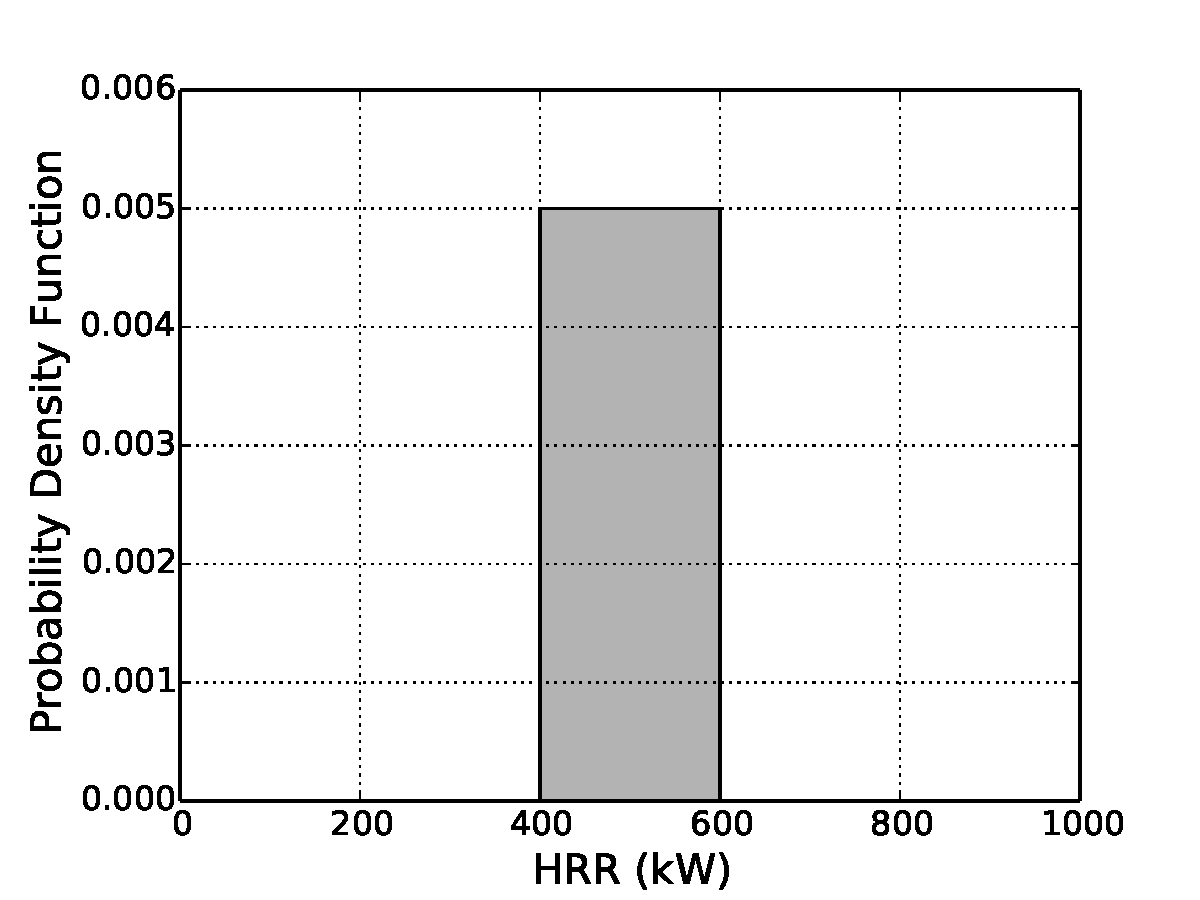
\includegraphics[width=2.6in]{Figures/input_PDF}
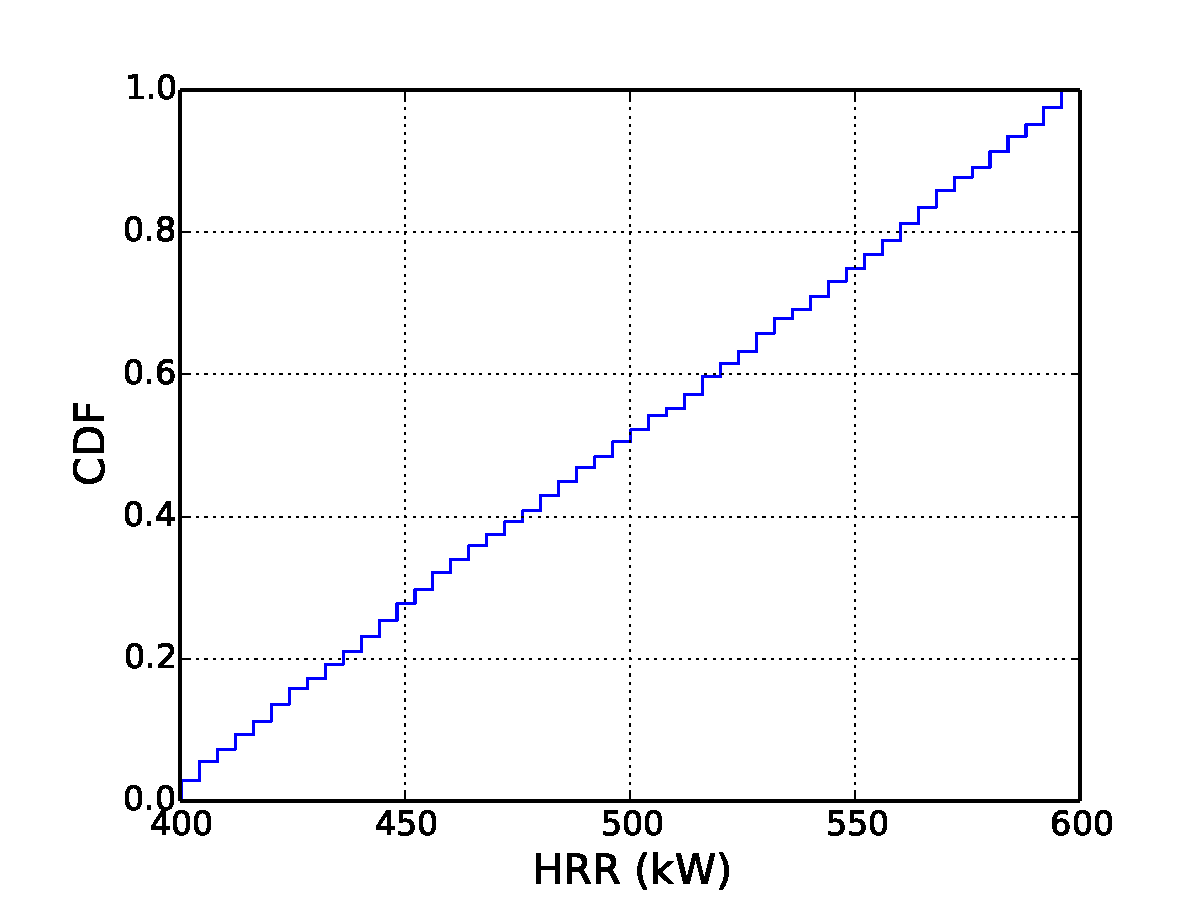
\includegraphics[width=2.6in]{Figures/input_CDF}
\caption{PDF and CDF of input HRR distribution}
\label{fig:case_3_input_distributions}
\end{figure}

The results of Case 2 are shown in Fig.~\ref{fig:case_3_output_distributions}.

\begin{figure}[!ht]
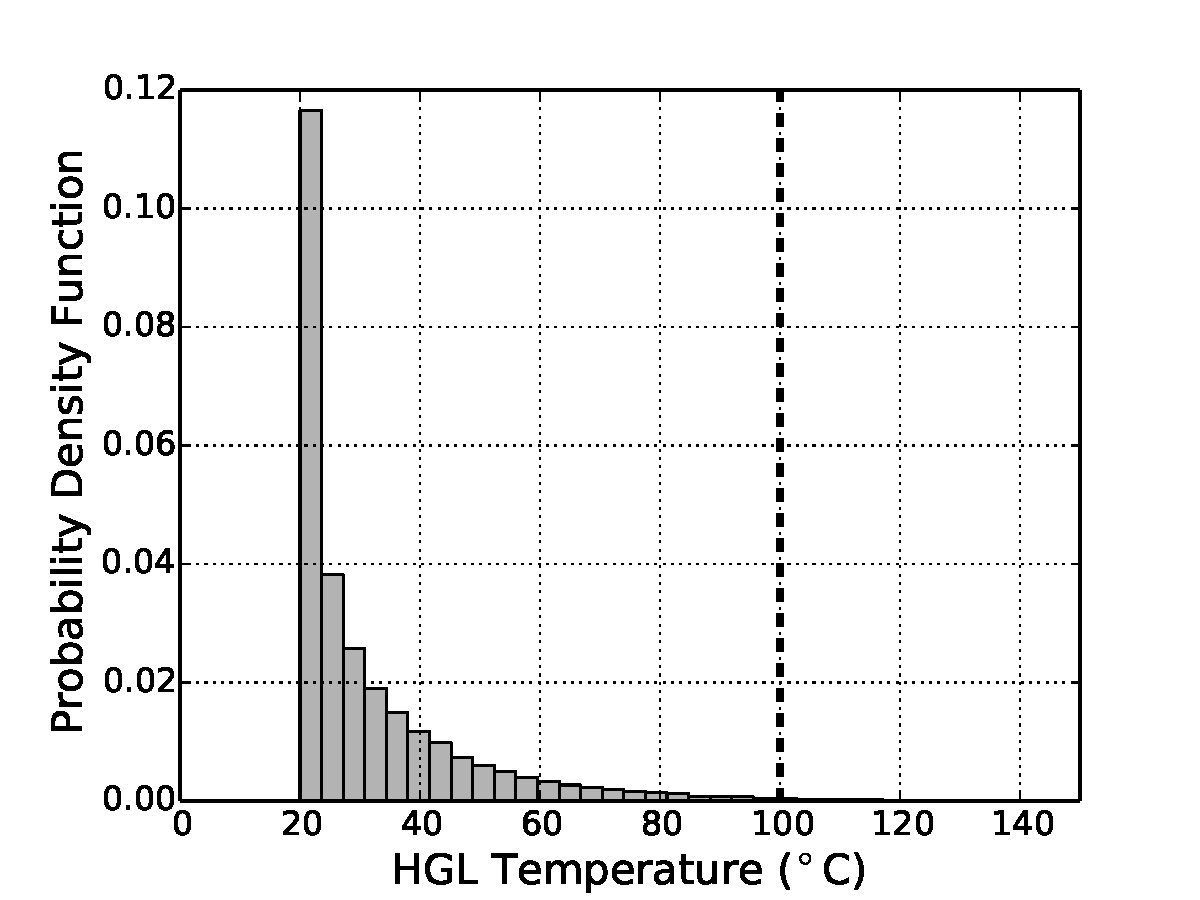
\includegraphics[width=2.6in]{Figures/output_PDF_3_combined}
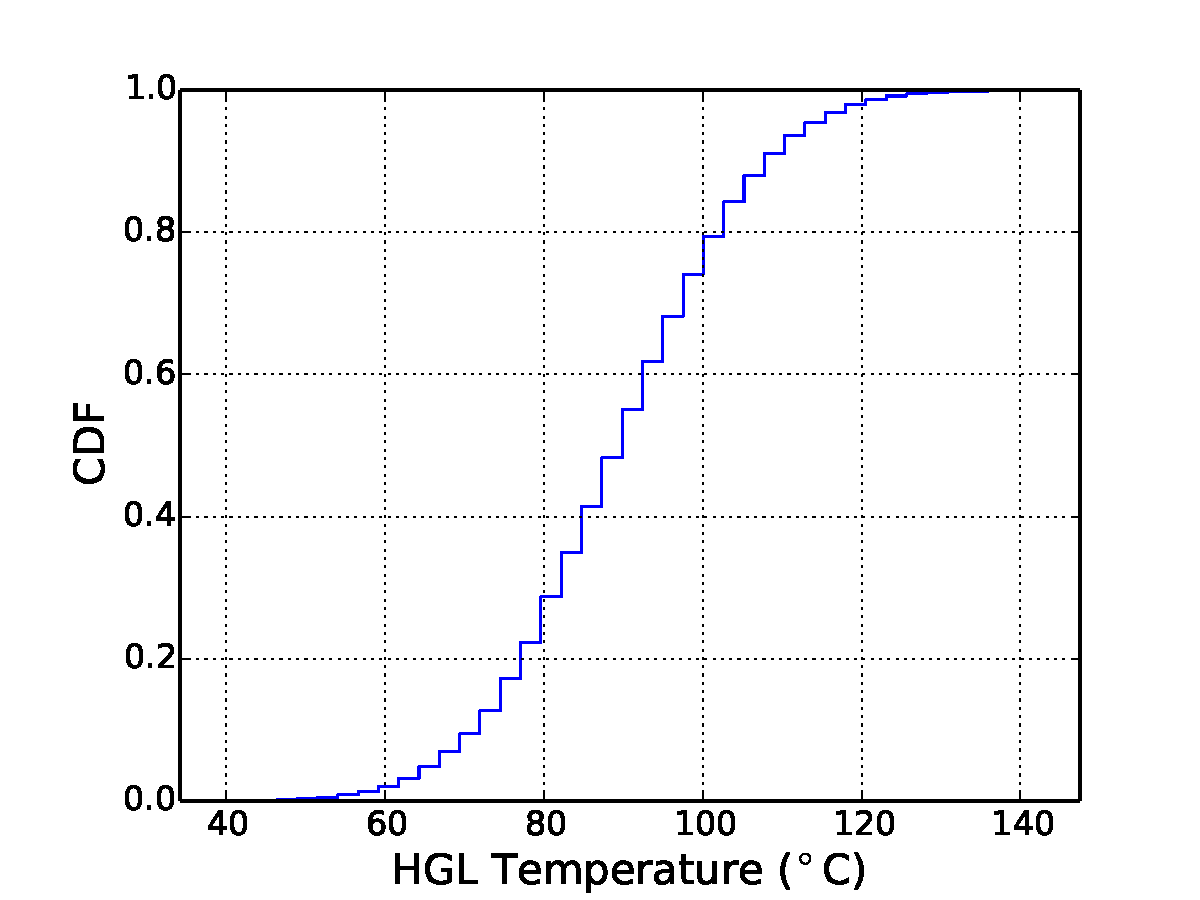
\includegraphics[width=2.6in]{Figures/output_CDF_3_combined}
\caption{PDF and CDF of output HGL temperature distribution}
\label{fig:case_3_output_distributions}
\end{figure}

For Case 3, the probability of exceeding the critical HGL temperature of 100~$^\circ$C is calculated as XX.


\section{Conclusions}
\label{sec:conclusions}


\bibliographystyle{unsrt}
\bibliography{references}

\end{document}